\section{Evaluation}
\label{sec:eval}

The goal of our study is to understand how \unsafe{} is used in open-source projects, and what the implications of this on the security of Go applications are. 
To achieve this, we answer the following research questions:

\begin{enumerate}[leftmargin=*,label={RQ\arabic*}]
    \item How many projects use \unsafe{} in Go code in their application? \label{rq:prevalApp}
    \item How many projects introduce \unsafe{} through their dependencies? \label{rq:prevalDeps}
    \item How deep in the import stack are the most imported \unsafe{} code packages? \label{rq:depsDepth}
    \item Which \unsafe{} keywords are used most? \label{rq:distTypes}
    \item What \unsafe{} operations are used in practice, and what is their goal? \label{rq:purpose}
    
    %\item Are there problems arising from the use of \unsafe{} that can lead to exploitable vulnerabilities? \label{rq:probsUnsafe}
\end{enumerate}

Figure~\ref{fig:overview} provides an overview of our study methodology.

\begin{figure*}[!t]
    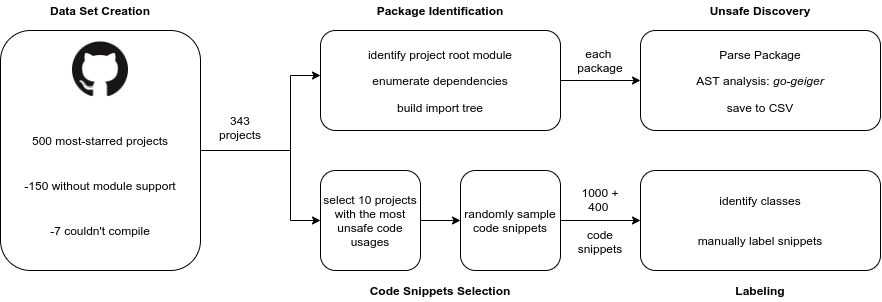
\includegraphics[width=\textwidth]{gfx/figures/overview.png}
    \caption{Overview of our Methodology and Empirical Results.}
    \label{fig:overview}
\end{figure*}



\subsection{Data Set Creation}

To answer our research question, we create a data set of open-source Go code available on GitHub.
As our research is focused on projects, we decide to crawl the \initalProjs{} most-stared Go projects available on GitHub. 
To further understand the influence of the dependencies, we selected the applications supporting \textit{go modules}.
With the introduction of Go \checkNum{1.13}, \textit{go modules} are the way to include dependencies within a Go application with the help of the Go tool chain. 
Unfortunately, \withoutModules{} of the projects did not yet support Go modules and we had to exclude them.
We further, had to remove \notCompiled{} projects as we couldn't compile those.
As a result, we end up with \projsAnalyzed{} top-rated Go projects collected from GitHub. 

\aw{Perhaps, we want to include some star stats or similar stats to show that we have relevant Go projects.}


\subsection{Unsafe Usages in Projects and Dependencies}

Answers to \ref{rq:prevalApp} and \ref{rq:prevalDeps}:

\checkNum{3355} of \checkNum{61839} (\checkNum{5.43\%}) transitively imported packages use unsafe. This answers \ref{rq:prevalDeps}

Number of projects: \checkNum{343}

Projects with $\geq 1$ unsafe project package: \checkNum{131} (\checkNum{38.19\%})

Projects with $\geq 1$ unsafe dependency: \checkNum{299} (\checkNum{87.17\%})

Projects with $\geq 1$ unsafe anywhere: \checkNum{312} (\checkNum{90.96\%})


\subsection{Import Depth of Unsafe}

Figure~\ref{fig:unsafe-import-depth} shows the number of packages with at least one \unsafe{} usage by its import depth for every project at its own, alongside the distribution for all projects combined. This answers~\ref{rq:depsDepth}

We see that most of the packages are imported early in the import stack with an average import depth of \averageUnsafeImportDepth (standard deviation of \stdUnsafeImportDepth).
Therefore, these packages can be manually found and evaluated with tolerable effort.

\begin{figure*}[!t]
    \vspace{2mm}
    \centering
    %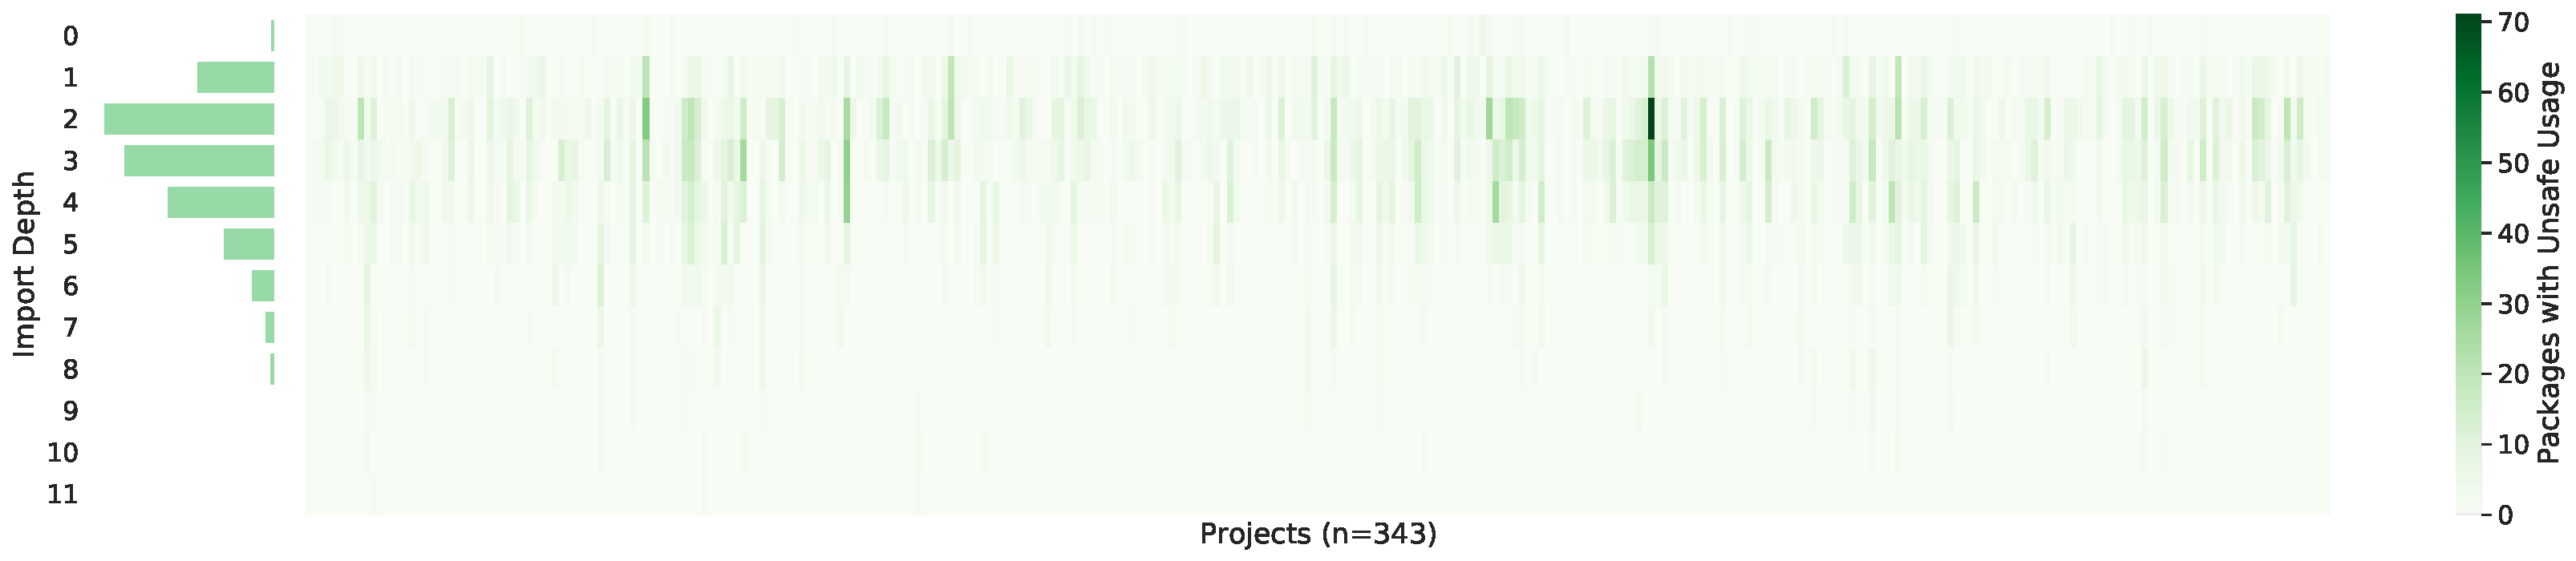
\includegraphics[width=\textwidth]{gfx/figures/unsafe-import-depth.pdf}
    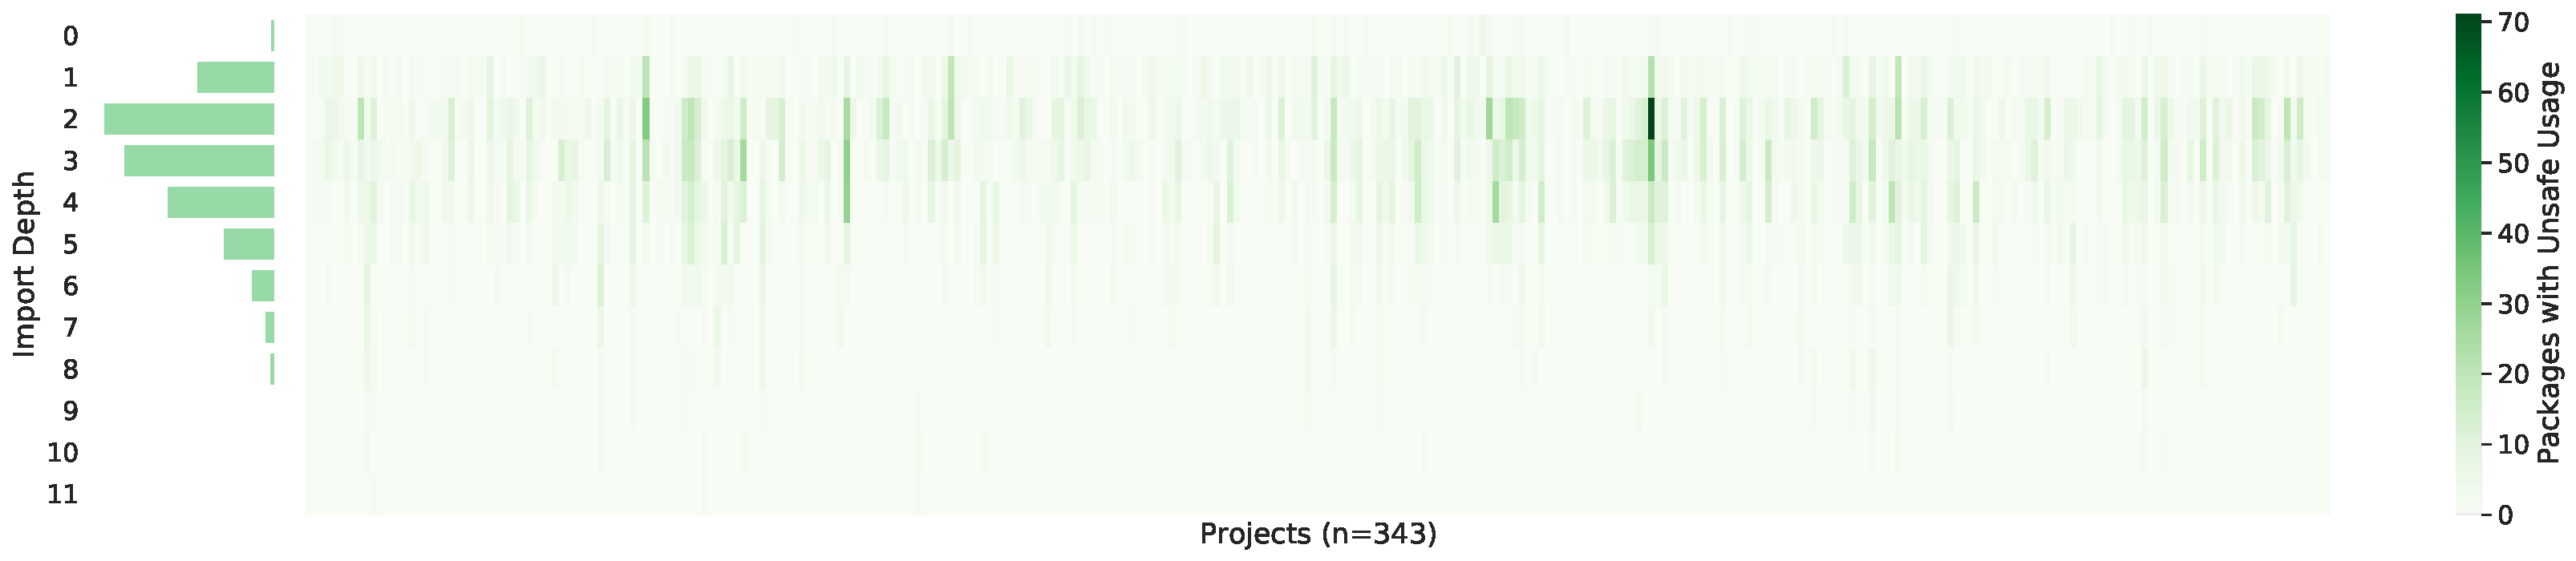
\includegraphics[width=.9\textwidth]{gfx/figures/unsafe-import-depth.pdf}
    \caption{Import Depth of Unsafe Packages. Unsafe packages are around a depth of \averageUnsafeImportDepth{} (sd=\stdUnsafeImportDepth{})}
    \label{fig:unsafe-import-depth}
    %\vspace{-10pt}
\end{figure*}



\subsection{Types of Unsafe}

To answer~\ref{rq:distTypes}, we show the distribution of the different \unsafe{} token types among the analyzed projects in Figure~\ref{fig:unsafe-tokens-distribution}.

For this figure, we duplicated packages by their name, module, and version. Packages that are imported in different versions by the projects in our data set are therefore counted once per version, because different version have potentially different \unsafe{} usages and coexist in the wild.

\begin{figure}[!t]
    \centering
    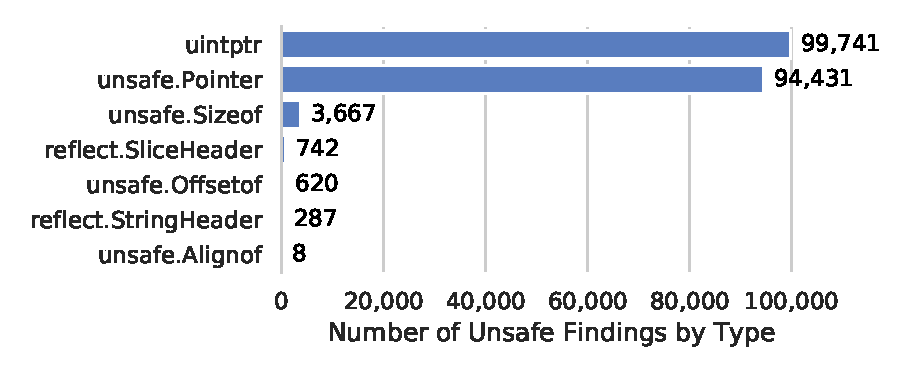
\includegraphics[width=0.43\textwidth]{assets/plots/distribution-unsafe-types.pdf}
    \caption{Distribution of different types of unsafe tokens}
    \label{fig:unsafe-tokens-distribution}
\end{figure}


\subsection{Purpose of Unsafe in Practice}

To answer~\ref{rq:purpose}, we present a summary of our labeled data set consisting of \checkNum{1,400} code snippets from the \checkNum{10} projects shown in Table~\ref{tbl:dataset-projects} in Table~\ref{tbl:dataset-classes}.

\begin{table}[h]
    \centering
    \caption{Selected projects for creation of the labeled data set}
    \label{tbl:dataset-projects}
    \begin{tabular}{llrrll}
    \hline
        {}  &                                               Name &  Stars &  Forks &   Revision \\ \hline
        1   &                              kubernetes/kubernetes &  66512 &  23806 &  fb9e1946b0 \\
        2   &                       mattermost/mattermost-server &  18277 &   4157 &  e83cc7357c \\
        3   &                                    rancher/rancher &  14344 &   1758 &  56a464049e \\
        4   &                                   weaveworks/scope &   4354 &    554 &  bf90d56f0c \\
        5   &                                          rook/rook &   7208 &   1472 &  ff90fa7098 \\
        6   &                                      elastic/beats &   8852 &   3207 &  df6f2169c5 \\
        7   &                                hashicorp/terraform &  22151 &   5729 &  01f91316da \\
        8   &                                      cilium/cilium &   5501 &    626 &  9b0ae85b5f \\
        9   &                                       grafana/loki &   9537 &    922 &  10a1f28a85 \\
        10  &                                  gorgonia/gorgonia &   3373 &    301 &  5fb5944d4a \\
        \hline
    \end{tabular}
\end{table}

We select the top \checkNum{10} projects with the most unsafe usages in non-standard library packages.
These projects, including the revision that we analyzed, are shown in Table~\ref{tbl:dataset-projects}.

From these projects and all their transitive dependencies, we randomly sample \checkNum{1000} application code and \checkNum{400} standard library code snippets. We define application code as all packages that are not part of the Go standard library or the \textit{golang.org/x/sys} module, as this module contains similar abstractions and code usages as the standard library. We split the snippets to analyze whether there is a difference in use between the two.

Then, we identify class labels in two dimensions: what is being done, and for what purpose. Finally, we manually label all \checkNum{1,400} code snippets.

\begin{table*}[htp!]
    \centering
    \caption[Labeled unsafe.Pointer usages in application code (non standard library) and standard library samples]
        {Labeled unsafe.Pointer usages in application code (non standard library) and standard library samples~\newline \tiny ~\newline \footnotesize
        \underline{eff}: efficiency, \underline{ser}: (de)serialization, \underline{gen}: generics,
        \underline{no GC}: avoid garbage collection, \underline{atomic}: atomic operations,
        \underline{FFI}: foreign function interface, \underline{HE}: hide from escape analysis, \underline{layout}: memory layout control,
        \underline{types}: Go type system,
        \underline{reflect}: type reflection, \underline{unused}: declared but unused \tiny ~\newline}
    \label{tbl:dataset-classes}
    \begin{adjustbox}{max width=\textwidth}
    
    %% do not paste from notebook, local changes done!
\begin{tabular}{r|cc|cc|cc|cc|cc|cc|cc|cc|cc|cc|cc|cc}
                    & \multicolumn{2}{c|}{\textbf{eff}} & \multicolumn{2}{c|}{\textbf{ser}} & \multicolumn{2}{c|}{\textbf{gen}} & \multicolumn{2}{c|}{\textbf{no GC}} & \multicolumn{2}{c|}{\textbf{atomic}} & \multicolumn{2}{c|}{\textbf{FFI}} & \multicolumn{2}{c|}{\textbf{HE}} & \multicolumn{2}{c|}{\textbf{layout}} & \multicolumn{2}{c|}{\textbf{types}} & \multicolumn{2}{c|}{\textbf{reflect}} & \multicolumn{2}{c|}{\textbf{unused}} & \multicolumn{2}{c}{\textbf{total}} \\ %\hline
                    &  \textbf{app} &  \textbf{std} &  \textbf{app} &  \textbf{std} &  \textbf{app} &  \textbf{std} &   \textbf{app} &  \textbf{std} &    \textbf{app} &  \textbf{std} &  \textbf{app} &  \textbf{std} &  \textbf{app} &  \textbf{std} &    \textbf{app} &  \textbf{std} &   \textbf{app} &  \textbf{std} &     \textbf{app} &  \textbf{std} &    \textbf{app} &  \textbf{std} &   \textbf{app} &  \textbf{std} \\ \hline
                    
                    \textbf{cast} & 562 & 16 & 178 & 33 & 18 & & & & & & 24 & 6 && 2 & 3 & 13 & & 45 & 1 & & & & 786 & 115 \\ 
      %  cast-struct &  401 &    4 &   50 &    6 &    6 &      &       &      &        &      &    6 &    2 &      &    2 &        &    4 &       &   31 &         &      &        &      &   463 &   49 \\
%\rowcolor{verylightgray}
      %   cast-basic &   90 &    2 &   29 &    3 &    1 &      &       &      &        &      &    1 &    3 &      &      &      2 &    7 &       &    1 &         &      &        &      &   123 &   16 \\
      %  cast-header &   36 &    1 &    3 &      &    1 &      &       &      &        &      &      &      &      &      &        &      &       &    3 &         &      &        &      &    40 &    4 \\
%\rowcolor{verylightgray}
      %   cast-bytes &   22 &    1 &   81 &   11 &      &      &       &      &        &      &    1 &      &      &      &      1 &      &       &    1 &         &      &        &      &   105 &   13 \\
      % cast-pointer &   13 &    8 &   15 &   13 &   10 &      &       &      &        &      &   16 &    1 &      &      &        &    2 &       &    9 &       1 &      &        &      &    55 &   33 \\
\rowcolor{verylightgray}
      \textbf{memory-access} &    2 &    1 &    9 &      &      &      &       &      &        &      &      &    1 &      &      &      4 &    6 &       &    4 &         &      &        &      &    15 &   12 \\
 \textbf{pointer-arithmetic} &    7 &    2 &    6 &    1 &      &      &       &      &        &    1 &      &    3 &    1 &    2 &      3 &    8 &       &    9 &         &      &        &      &    17 &   26 \\
\rowcolor{verylightgray}
         \textbf{definition} &    4 &    1 &   23 &      &    2 &      &       &      &        &      &    4 &    5 &      &      &        &    9 &       &    8 &       6 &    3 &        &      &    39 &   26 \\
           \textbf{delegate} &    4 &      &   64 &      &    2 &      &       &      &     11 &    5 &   29 &   45 &      &    4 &        &   14 &       &    6 &         &    1 &        &      &   110 &   75 \\
\rowcolor{verylightgray}
            \textbf{syscall} &      &      &      &      &      &      &    17 &  138 &        &      &      &      &      &      &        &      &       &      &         &      &        &      &    17 &  138 \\
             \textbf{unused} &      &      &      &      &      &      &       &      &        &      &      &      &      &      &        &      &       &      &         &      &     16 &    8 &    16 &    8 \\ \hline
%\rowcolor{verylightgray}
                  \textbf{total} &  579 &   20 &  280 &   34 &   22 &    0 &    17 &  138 &     11 &    6 &   57 &   60 &    1 &    8 &     10 &   50 &     0 &   72 &       7 &    4 &     16 &    8 &  1000 &  400 \\
\end{tabular}

    \end{adjustbox}
        \vspace{-10pt}
\end{table*}

We see that...